\documentclass{beamer}
 
\usepackage[utf8]{inputenc}
\usepackage{graphicx,amsmath,amsthm, amssymb,setspace, mathtools}
\usepackage{dirtytalk}
 \usepackage{graphicx}
 \graphicspath{ {images/} }
 
 \def\DM{\protect{$\cal{DM}$}}
 \def\interior{\protect{\textnormal{ri}}}
 \def\relint{\protect{\textnormal{ri}}}
 \def\closure{\protect{\textnormal{closure}}}
 \def\rank{\protect{\textnormal{rank}}}
 \def\diagonal{\protect{\textnormal{diag}}}
 
%Information to be included in the title page:
\title{Sample title}
\author{Anonymous}
\institute{ShareLaTeX}
\date{2014}
 
 
 \title[About Beamer] %optional
 {Design and implementation of a homogeneous interior-point method for conic programming involving exponential cone constraints}
 
 
 \author[gaoyuan] % (optional, for multiple authors)
 {Yuan Gao$^1$ \\[1ex] Supervised by \\[0.5ex] Prof. Kim-Chuan Toh$^1$\\Prof. Melvyn Sim$^2$}
 
 \institute[VFU] % (optional)
 {
 	$1$ Department of Mathematics, National University of Singapore\\
 	$2$ Department of Decision Sciences, National University of Singappore
 }
 
\date % (optional)
{Honour's Project Introductory Talk\\ Oct 2016}
 
 
\begin{document}
 
\frame{\titlepage}
 
\begin{frame}
\frametitle{Contents}
\begin{itemize}
	\item Introduction, motivation and preliminaries.
	\item Current implementation.
	\item Examples of application.
	\begin{itemize}
		\item Optimizing the satisficing measure.*
		\item Convex approximation of chance constrained problems.
		\item Robust choice model.
	\end{itemize}
		\item The algorithm.
	\begin{itemize}
		\item The standard conic form.
		\item A homogeneous self-dual model.
		\item The central path and search directions.
		\item Methods for solving the linear systems.*
		\item Termination conditions.
	\end{itemize}
	\item Plans for the next step.
\end{itemize}
\small{$*$ Optional contents. Will be briefly covered if time permits.}
\end{frame}

\begin{frame}
\frametitle{Introduction}
\begin{itemize}
\item Many interesting real-world problems can be modeled as \textit{convex optimization} problems.
	\begin{itemize}
		\item More specifically, LP, SOCP and SDP problems.
	\end{itemize}
\item \textit{In theory}, these problems can be \textit{efficiently} solved by a class of algorithms known as \textit{interior-point methods} (IPM).
	\begin{itemize}
		\item Kamarkar (1984) first proposed and studied IPM for LP.
	\end{itemize}
\item Powerful solvers have been developed since then.
	\begin{itemize}
		\item LP: Excel, Matlab, AMPL.
		\item SOCP/MISOCP: Cplex, Gurobi.
		\item SDP: SDPT3 (Toh, Todd \& T\"ut\"unc\"u), SeDuMi (Sturm, Romanko \& Pólik).
	\end{itemize}
\end{itemize}
\end{frame}

\begin{frame}
	\frametitle{Motivation}
	\begin{itemize}
		\item Recently, researchers in OR, Econometrics and EECS have been considering (convex) optimization models that cannot be formulated as LP, SOCP or SDP.
		\begin{itemize}
			\item Only small and \say{nice} instances can be solved (through LP/SOCP approximation and caling the respective solvers).
		\end{itemize}
		\item Models with $\log$ and $\exp$ functions in their objectives and constraints can be formulated as conic programming problems involving \textit{exponential cone constraints}.
		\begin{itemize}
			\item They can potentially be solved efficiently by IPM.
		\end{itemize}
	\end{itemize}
\end{frame}

\begin{frame}
	\frametitle{Motivation}
	\begin{itemize}
		\item There have been a few works on both theoretical and computational aspects of IPM for \textit{non-symmetric conic programming}.
		\begin{itemize}
			\item Nesterov (2006).
			\item Charles and Glineur (2009).
			\item Ye and Skajaa (2015).
		\end{itemize}
		\item We need a solver/program that efficiently solves problems involving exponential cone constraints.
		\begin{itemize}
			\item An important class of non-symmetric conic programming problems.
		\end{itemize}
	\end{itemize}
\end{frame}

\begin{frame}
	\frametitle{Preliminaries}
	\begin{itemize}
		\item Notations.
		\begin{itemize}
			\item $\mathbb{R}_+ = \left\{x\in \mathbb{R} \mid x\geq 0  \right\}$. \\[1ex]
			\item $\mathcal{Q}^p = \left\{\left(x_1, \cdots, x_p\right)^T \in \mathbb{R}^p \mid x_1 \geq \sqrt{x_2^2+\cdots+x_p^2}\right\}$. \\[1ex]
			\item $\mathcal{K}^0_{\exp} = \left\{ \left(x,y,z\right)^T\in \mathbb{R}^3 \ \rvert\ z>0, \exp\left(\dfrac{x}{z} \right)\leq\dfrac{y}{z} \right\}$. \\[1ex]
			\item $\mathcal{K}_{\exp}=\textnormal{closure} \left(\mathcal{K}^0_{\exp} \right)$.\\[2ex]
		\end{itemize}
	\item It can be shown that 
	\[\mathcal{K}_{\exp} = \mathcal{K}^0_{\exp} \cup \left(-\mathbb{R}_+\right)\times \mathbb{R}_+ \times \left\{0\right\}. \]
	\item More notations and definitions are needed when discussing the algorithm.
	\end{itemize}
\end{frame}

\begin{frame}
	\frametitle{Current implementation}
	\begin{itemize}
		\item We developed a program that \textit{solves} problems coded in the following form
		\begin{align*}
		\begin{split}
		\quad &\min_{x_1, \cdots, x_N}\,\, \sum_{i=1}^N c_i^Tx_i\\
		& \text{s.t.}\,\, \sum_{i=1}^N A_i x_i = b,\ x_i \in K_i, \forall i
		\end{split} \quad\quad\quad\quad\quad\quad\quad\,\,\, \textnormal{(P*)}
		\end{align*}
		where $K_i\subset \mathbb{R}^{n_i}$ is one of the following.
		\begin{itemize}
			\item nonnegative orthant $\mathbb{R}_+^{n_i}$.
			\item product of second-order cones $\mathcal{Q}^{q_1}\times \cdots \times \mathcal{Q}^{q_{k_i}}$, $\sum_{j=1}^{k_i} q_j = n_i$.
			\item product of the exponential cone  $\left(\mathcal{K}_{\exp}\right)^{k_i}$, $3k_i = n_i$.
			\item unrestricted space $\mathbb{R}^{n_i}$.
		\end{itemize}
		\item To solve a general convex optimization model involving $\log$ and $\exp$ functions, it has to be converted into (P*).
	\end{itemize}
\end{frame}

\begin{frame}
	\frametitle{Current implementation}
	\begin{itemize}
		\item For $x_i\in \mathbb{R}^{n_i}$, let $x_i = x_i^+ - x_i^-$, where $x_i^+, x_i^- \in \mathbb{R}_+^{n_i}$.
		\item Therefore (P*) can be converted into the following \textit{standard conic form}
		\begin{align*}
		\begin{split}
		\quad &\min_x\,\, c^Tx\\
		& \text{s.t.}\,\, A x = b,\ x \in \mathcal{K}
		\end{split} \quad\quad\quad\quad\quad\quad\quad\,\,\, \textnormal{(P)}
		\end{align*}
		where $ \mathcal{K} = \mathbb{R}^{n_l} \times \left(\mathcal{Q}^{q_1}\times\cdots\times \mathcal{Q}^{q_{m}}\right)\times \left(\mathcal{K}_{\exp}\right)^h$,
		$n_q = q_1 + \cdots + q_m$, $n_e = 3h$, $n=n_l+n_q+n_e$, $A\in \mathbb{R}^{m\times n}$, $x\in \mathbb{R}^n$.
	\end{itemize}
\end{frame}

\begin{frame}
	\frametitle{Example: Asset allocation via satisficing measure}
	\begin{itemize}
		\item Brown, Giorgi and Sim (2009) consider the following entropic prospective satisficing measure (EPSM) of a random variable $\boldsymbol{X}$,
		\[\rho(\boldsymbol{X}) = \sup \left\{t\in \mathbb{R}\backslash \left\{0\right\} \ \big\rvert\ \dfrac{1}{t}\log \mathbb{E} \left[\exp\left(-t\boldsymbol{X}\right)\right] \leq 0 \right\}. \]
	\end{itemize}
\end{frame}

\begin{frame}
	\frametitle{Example: Asset allocation via satisficing measure}
	\begin{itemize}
		\item Suppose there are $n$ assets with independent random returns $V_i\in \left\{v^l_i, v^h_i \right\}$, $v^l_i\leq v^h_i$, $\mathbb{P}\left(V_i = v^j_i\right) = p^q_i$, $q=h,l$, $p^h_i+p^l_i=1$, $i=1,\cdots, n$.
		\item Consider the following asset allocation problem, with a target return $\tau < \max_{1\leq j\leq n} \mathbb{E}\left(V_j\right),$
		\begin{align} \label{satisficing_original}
		\begin{split}
		& \mathcal{O}^{EPSM} = \\
		& \sup_{w_1, \cdots, w_n} \rho\left(\sum_{i=1}^n w_iV_i - \tau\right) \\
		& \textit{s.t.}\ \sum_{i=1}^n w_i = 1,\ w_i\geq 0,\forall i.
		\end{split}
		\end{align}
		\begin{itemize}
			\item This example is for illustration purpose.
		\end{itemize}
	\end{itemize}
\end{frame}

\begin{frame}
	\frametitle{Example: Asset allocation via satisficing measure}
	\begin{itemize}
		\item Problem \eqref{satisficing_original} can be formulated into (P*) as follows.
		\begin{align}\label{epsm_std_form_minimization}
		\begin{split}
		\mathcal{O}^{'} = &\min\ \ a_1^l \\
		\textnormal{s.t.}\quad &\sum_{j=1}^n z_j = -\tau,\ \sum_{j=1}^n w_j = 1, \\
		& p_j^l s_j^l +p_j^h s_j^h - a_j = 0,\ j=1,\cdots,n, \\
		& u_j^q + z_j + v_j^q w_j = 0,\ q=l,h,\ j = 1,\cdots, n, \\
		& a^l_1 - a^h_1 =0,\ a^q_1 - a^q_j = 0,\ q=l,h,\ j = 2, \cdots, n, \\
		\end{split}
		\end{align}
		with decision variables
		\begin{align*}
		&\left(u_j^q, s_j^q, a_j^q\right) \in \mathcal{K}_{\exp},\ q = l,h,\ j=1,\cdots,n, \\
		&\left(w_1,\cdots,w_n\right)^T\in \mathbb{R}_+^n,\ \left(z_1,\cdots,z_n\right)^T \in \mathbb{R}^n.
		\end{align*}
	\end{itemize}
\end{frame}

\begin{frame}
	\frametitle{Example: Asset allocation via satisficing measure}
	\begin{itemize}
		\item Note that $\mathcal{O}^{EPSM} = 1/\mathcal{O}^{'}>0$.
		\item To solve a feasible instance with $n= 1000$, our solver takes less than 3 minutes (on a modest laptop) while SOCP approximation becomes impractical.
		\begin{itemize}
			\item The resulting SOCP instances are extremely large.
			\item The approximate solution may not converge.
		\end{itemize}
	\end{itemize}
\end{frame}

\begin{frame}
	\frametitle{Example: Convex approximation of chance constrained problems}
	\begin{itemize}
		\item Chance constrained problems arise naturally in OR models. 
		\begin{itemize}
			\item Chance constraints look like $\mathbb{P}\left(F\left(\boldsymbol{x},\tilde{\boldsymbol{\xi}}\right)\leq 0\right)\geq 1-\alpha$, where $\boldsymbol{x}$ is the decision vector, $\tilde{\boldsymbol{\xi}}$ is a random vector and $\alpha$ is a given \say{confidence level.}
		\end{itemize}
		\item In general, they are very difficult to solve/approximate.
	\end{itemize}
\end{frame}

\begin{frame}
	\frametitle{Example: Convex approximation of chance constrained problems}
	\begin{itemize}
			\item The scenario approach (based on Monte Carlo simulation) can be used to approximate problems with \say{nice} structures (Nemirovski \& Shapiro, 2005).
			\begin{itemize}
				\item In general, the solution yielded is not feasible under the original chance constraints.
				\item It is difficult to establish \textit{risk bounds}.
				\item A reasonably reliable solution requires a huge number of realizations of $\tilde{\boldsymbol{\xi}}$.
			\end{itemize}
	\end{itemize}
\end{frame}

\begin{frame}
	\frametitle{Example: Convex approximation of chance constrained problems}
	\begin{itemize}
		\item Nemirovski and Shapiro (2006) developed a \textit{conservative} approximation scheme named the \textit{Bernstein approach}, which has several advantages compared to the scenario approach.
		\begin{itemize}
			\item Given a \say{nice} chance constrained problem (P1) with information about the random variables, define an associated convex optimization problem (P2).
			\item (P2) can be solved efficiently (at least in theory).
			\item The solution to (P2) is always feasible to (P1).
			\item The optimal objective value of (P2) is (usually) suboptimal to (P1).
		\end{itemize}
	\end{itemize}
\end{frame}

\begin{frame}
	\frametitle{Example: Convex approximation of chance constrained problems}
	\begin{itemize}
		\item Consider the following asset allocation problem
		\begin{align} \label{investment_problem}
		\begin{split}
		& \mathcal{O}^{chance}\quad=\\
		&\max_{\begin{matrix}
			\tau \in \mathbb{R}\\ 	
			x_0, x_1\cdots,x_n \geq 0
			\end{matrix}}\ (\tau - 1)\ \ \\ 
		& \textnormal{s.t.}\ \ \mathbb{P} \left(\tau > \sum_{j=0}^n \tilde r_j x_j \right) \leq \alpha,\ \sum_{j=0}^{n} x_j \leq 1
		\end{split}
		\end{align}
		where $\tilde{r}_j$ is the random return of asset $j$, $j=0\cdots,n$ and $\alpha \in [0,1]$ denotes the confidence level.
	\end{itemize}
\end{frame}

\begin{frame}
	\frametitle{Example: Convex approximation of chance constrained problems}
	\begin{itemize}
		\item We characterize $\tilde{r}_j,\ j=0,\cdots,n$ as follows.
		\begin{enumerate}
			\item The returns satisfy $\tilde r_0=r_0=1$, $\mathbb{E}(\tilde r_j) = 1 + \rho_j,\ j=1,\cdots,n$.
			
			\item For $j=1,\cdots,n$,  $l=1,\cdots,q$, let $\tilde r_j = \tilde\eta_j + \sum_{l=1}^q \gamma_{jl}\tilde\zeta_l$ where $\tilde\eta_j \sim \mathcal{LN}(\mu_j, \sigma_j^2)$, $\tilde\zeta_l \sim \mathcal{LN}(\nu_l, \theta_l^2)$ ($\mathcal{LN}$ denotes lognormal distribution).\\[1ex]
			
			\item All $\tilde\eta_j$ and $\tilde\zeta_l$ are mutually independent.
			
			\item The parameters $\rho_j$, $\mu_j$, $\sigma_j$, $\nu_j$, $\theta_j$, $\gamma_{jl}$ satisfy
			\begin{align*}
			&\mu_j, \nu_j, \gamma_{jl} \geq 0,\ 0\leq \rho_1 \leq \cdots \leq \rho_n,\\[1ex]
			&\mathbb{E}\left[\sum_{l=1}^q \gamma_{jl} \tilde\zeta_l\right] =  \sum_{l=1}^q \gamma_{jl} \exp \left(\nu_l + \dfrac{\theta_l^2}{2}\right) = \dfrac{\rho_j}{2},\\[1ex]
			&\mathbb{E}\left[\tilde\eta_j\right] = \exp\left(\mu_j + \dfrac{\sigma_j^2}{2}\right) = 1 + \dfrac{\rho_j}{2},\ j =1,\cdots, n.
			\end{align*}
		\end{enumerate}
	\end{itemize}
\end{frame}

\begin{frame}
	\frametitle{Example: Convex approximation of chance constrained problems}
	\begin{itemize}
	\item To apply the approximation scheme, the $\mathcal{LN}$ random variables $\tilde \eta_j$, $\tilde \gamma_l$ need to be discretized (rounded from below) so that their moment generating functions (MGF) are well defined. 
	\item Assume this has been done without change of notation.
	\end{itemize}
\end{frame}

\begin{frame}
	\frametitle{Example: Convex approximation of chance constrained problems}
	\begin{itemize}
	\item Let $q=n+d$, $\bar{\boldsymbol{x}}=(x_0, x_1, \cdots, x_n)$,
	\[g_0(\bar{\boldsymbol{x}}) = \tau - x_0,\]
	\[\tilde{\xi}_j = \tilde{\eta}_j,\ g_j(\bar{\boldsymbol{x}}) = -x_j,\ j=1,\cdots, n,\] 
	\[\tilde{\xi}_{n+l} = \tilde{\zeta}_l,\ g_{n+l}(\bar{\boldsymbol{x}}) = -\sum_{j=1}^n \gamma_{jl}x_j,\ l=1,\cdots,q.\]
	\item For each $j$, $k=1, \cdots, N_j$, let $\tilde{\xi}_j \in \left\{v_k^j \mid k=1,\cdots, N_j \right\}$ and $\mathbb{P}\left(\tilde{\xi}_j = v_k^j\right) = p_k^j$. Let $M_j: z \rightarrow \sum_{k=1}^{N_j} p_k^j \exp \left(v_k^j z\right)$ be the MGF of $\tilde{\xi}_j$ and denote $\Lambda_j(\cdot) = \log M_j(\cdot)$.
	\begin{itemize}
		\item Values of $v^j_k$, $p^j_k$ are determined by the parameters of the $\mathcal{LN}$ distributions and the discretization scheme.
	\end{itemize}
	\end{itemize}
\end{frame}

\begin{frame}
	\frametitle{Example: Convex approximation of chance constrained problems}
	\begin{itemize}
		\item The Bernstein approximation to \eqref{investment_problem} is 
		\begin{align} \label{Bernstein_approx_direct_form}
		\begin{split}
		&\mathcal{O}^{Bernstein}\quad =\quad \\
		&\max_{\begin{matrix}
			\tau \in \mathbb{R},\\ 	
			\bar{\boldsymbol{x}} = (x_0, x_1\cdots,x_n)^T \geq 0
			\end{matrix}} (\tau - 1)\ \ \ \\
		\textnormal{s.t.}\ & \inf_{t>0} \left(g_0(\bar{\boldsymbol{x}}) + \sum_{j=1}^d t \Lambda_j\left(t^{-1}g_j(\bar{\boldsymbol{x}})\right) - t\log \alpha \right) \leq 0,\\
		& \sum_{j=0}^n x_j \leq 1.\ \ 
		\end{split}
		\end{align}	
	\end{itemize}
\end{frame}

\begin{frame}
	\begin{itemize}
		\item It can be shown that \eqref{Bernstein_approx_direct_form} can be formulated into (P*) as
		\begin{align}
		\begin{split}\label{reformulated_std_conic_form}
		\mathcal{O}^{P} \quad = \quad &\min  -\tau \\ 
		\textnormal{s.t.}\ \ \ & x_0 + \sum_{j=1}^n x_j + s_x = 1,\ g_0 + \left(\sum_{j=1}^d s_j\right) - \left(\log \alpha\right) t_0 = 0, \\
		&\ g_0  - \tau + x_0 = 0,\  g_j + x_j = 0,\ j = 1, \cdots, n,\\ 
		& g_{n+l} + \sum_{j=1}^n \gamma_{jl} x_j = 0,\ l = 1, \cdots, q, \\
		& w_k^j - v_k^j g_j + s_j = 0,\ j = 1, \cdots,d,\ k = 1, \cdots, N_j, \\
		& \sum_{k=1}^{N_j} p_k^j u_k^j - t_0 = 0,\  j =1,\cdots,d, \\
		& t_0 - t_k^j = 0,\ j = 1,\cdots, d,\ k = 1,\cdots,N_j.
		\end{split}
		\end{align}
	\end{itemize}
\end{frame}

\begin{frame}
	with decision variables
	\begin{align*}
	& \tau \in \mathbb{R} \\
	& x_0, x_1, \cdots, x_n, s_x \geq 0 \\
	& g_0, g_1, \cdots, g_d \in \mathbb{R} \\
	& t_0 \geq 0 \\
	& s_1, \cdots, s_d \in \mathbb{R} \\
	& \left(w_k^j, u_k^j, t_k^j\right) \in \mathcal{K}_{\exp},\ j = 1, \cdots, d,\ k = 1,\cdots, N_j.
	\end{align*}
\end{frame}

\begin{frame}
	\frametitle{Example: Convex approximation of chance constrained problems}
	\begin{itemize}
		\item Define $\mathcal{O}^{nominal} = \max\left\{\rho_i \mid i=1,\cdots,n\right\} = \rho_n$.
		\begin{itemize}
			\item This is the optimal objective of \eqref{investment_problem} with all $\tilde{r}_i$ replaced by their respective means.
		\end{itemize}
		\item Note that $\mathcal{O}^{nominal}\geq\mathcal{O}^{chance} \geq \mathcal{O}^{Bernstein} = -\mathcal{O}^P - 1$.
	\end{itemize}
\end{frame}

\begin{frame}
	\frametitle{Example: Convex approximation of chance constrained problems}
	\begin{itemize}
		\item For a randomly generated instance of \eqref{Bernstein_approx_direct_form} with $n=100$, $q=4$, $\alpha=0.05$, $\epsilon=10^{-5}$, $\Delta=0.005$ and appropriate values of distributional parameters, the resulting standard form (P') has $A \in \mathbb{R}^{2187\times 3491}$, $density(A) = 0.0012058$,
		$N_l = 539$, $N_q = 0$, $N_e = 2952$.
		\item The dimension of (the exponential cone part of) $A$ depends chiefly on the \say{shape} of the $\mathcal{LN}$ distributions and precision of the discretization.
	\end{itemize}
\end{frame}

\begin{frame}
	\frametitle{Example: Convex approximation of chance constrained problems}
	\begin{itemize}
		\item Our solver took $13.65$ seconds to obtain an \say{optimal} solution.
		\item CVX (Grant and Boyd, 2013) took $255.65$ seconds before termination \textit{without} a solution.
		\begin{itemize}
			\item It is the most well developed algebraic modeling tool for specifying and solving convex optimization problems.
			\item It used successive approximation and called SDPT3 several times to solve the resulting SOCP instances. 
			\item These SOCP instances have very large dimensions.
			\item SOCP approximation scheme is not reliable in general, although SOCP solvers are very efficient and robust.
		\end{itemize}
		\item For smaller instances, CVX and our solve give the same solutions.
	\end{itemize}
\end{frame}

\begin{frame}
	\frametitle{Example: Convex approximation of chance constrained problems}
	\begin{itemize}
		\item The solution obtained through Bernstein approximation might be too conservative.
		\begin{itemize}
			\item The solution is \textit{too} reliable while the objective value is not satisfactory.
		\end{itemize}
		\item In practice, \textit{tuning} might be necessary.
		\begin{itemize}
			\item Set a large $\alpha'$ in (P1). 
			\item Find a solution to (P2) and approximate the \textit{empirical risk} $\alpha^*$ of the solution through simulation.
			\item Vary $\alpha'$ until $\alpha^*$ is \say{close} to $\alpha$.
		\end{itemize}
	\end{itemize}
\end{frame}

\begin{frame}
	\frametitle{Example: Robust choice model}
	\begin{itemize}
		\item Consider a customer and $J$ types of crackers.
		\item Each type of crackers has $Q$ attributes.
		\begin{itemize}
			\item For example, price, net weight, whether it is displayed in a conspicuous spot.
			\item Attributes might be \textit{collinear} (correlated).
		\end{itemize}
		\item The probability of the customer choosing type $j$ is
		\[ p_j = \dfrac{\exp\left(\alpha_j + \boldsymbol{x}_j' \boldsymbol{\beta} \right)}{ \sum_{l=1}^J \exp\left(\alpha_l + \boldsymbol{x}_l' \boldsymbol{\beta} \right) } \]
		where $\boldsymbol{x}_j$ denotes a vector of attribute values.
	\end{itemize}
\end{frame}

\begin{frame}
	\frametitle{Example: Robust choice model}
	\begin{itemize}
		\item Suppose we have some data.
		\begin{itemize}
			\item There have been $N$ (independent) purchases.
			\item For each purchase, the attributes of all types of crackers $\boldsymbol{X} = \left\{\boldsymbol{x}_{nj}\right\}\subset \mathbb{R}^Q$ and the customer's choice $\boldsymbol{Y} =\left(y_{nj}\right) \subset \left\{0,1\right\}^{N\times J}$ are recorded.
		\end{itemize}
		\item We want to find $\hat{\boldsymbol{\alpha}}$, $\hat{\boldsymbol{\beta}}$, estimates of $\boldsymbol{\alpha}$, $\boldsymbol{\beta}$.
		\begin{itemize}
			\item The classical approach is maximum-likelihood estimation, which is thoroughly discussed in Chapter 3 of Train's (2009) book \textit{Discrete Choice Methods with Simulation}.
		\end{itemize}
	\end{itemize}
\end{frame}

\begin{frame}
	\frametitle{Example: Robust choice model}
	\begin{itemize}
		\item We find $\hat{\boldsymbol{\alpha}}$, $\hat{\boldsymbol{\beta}}$ by solving the following optimization problem
		\begin{align}\label{robust_choice_model_max_min}
		\mathcal{O}^{rc} = \max_{\boldsymbol{\alpha}, \boldsymbol{\beta}}\ \ \min_{\left(z_{nj}\right)\in \mathcal{Z}\left(\Gamma\right)}\ \
		\sum_{n=1}^N \sum_{j=1}^J z_{nj} \log\dfrac{exp\left(\alpha_j + \boldsymbol{x}'_{nj}\boldsymbol{\beta}\right)}{\sum_{l=1}^J exp\left(\alpha_l + \boldsymbol{x}'_{nl}\boldsymbol{\beta}\right)}
		\end{align}
		where \[\mathcal{Z}\left(\Gamma\right) = \left\{\left(z_{nj}\right)\in \mathbb{R}_+^{N\times J} \ \bigg\rvert\ \begin{matrix}
		\sum_{j=1}^J z_{nj}=1,\forall n, \\[1ex]
		\sum_{n=1}^N z_{n\hat{\jmath}_n} \geq N - \Gamma \\
		\end{matrix} \right\}\]
		and $\hat{\jmath}_n$ is such that $y_{n\hat{\jmath}_n} = 1$ ($y_{nj}=0$ for $j\neq \hat{\jmath}_n $).
		\begin{itemize}
			\item The parameter $\Gamma$ accounts for \say{irrational} choices.
			\item Letting $\Gamma > 0$ usually yields \say{better} estimates by allowing customs to depart from their usual behavioral patterns occasionally.
		\end{itemize}
	\end{itemize}
\end{frame}

\begin{frame}
	\frametitle{Example: Robust choice model}
	\begin{itemize}
		\item By taking the dual of the inner minimization problem which is LP on $\left(z_{nj}\right)$, it can be shown that \eqref{robust_choice_model_max_min} is \textit{equivalent} to
		\begin{align}\label{robust_choice_dual_convex}
		\begin{split}
		\mathcal{O}^{rc}\quad  &=\quad 
		\\&\max_{\left(a_n\right),b, \boldsymbol{\alpha}, \boldsymbol{\beta}}\  \left(\sum_{n=1}^N a_n\right)+\left(N-\Gamma\right)b \\
		\textnormal{s.t.}\quad & a_n +  \mathbb{I}_{\left\{j=\hat{\jmath}_n\right\}}\cdot b \leq -\log \sum_{l=1}^J \exp\left(\alpha_l - \alpha_j + \left(\boldsymbol{x}_{nl}-\boldsymbol{x}_{nj_n}\right)'\boldsymbol{\beta}\right),\\ &\quad \quad \quad \quad \quad \quad \quad \quad \quad \quad n=1,\cdots, N,\ j=1,\cdots, J. \\
		\end{split}
		\end{align}
	\end{itemize}
\end{frame}

\begin{frame}
	\frametitle{Example: Robust choice model}
	\begin{itemize}
		\item Problem \eqref{robust_choice_dual_convex} can be formulated into (P*) and hence solved by our solver. 
		\item An instance of $N=3000$ ($J=4$, $Q=3$) can be solved to satisfactory accuracy in $10$ hours.
		\item CVX can only handle instances with $N\leq 150$, which can be loaded and solved in minutes by our solver.
	\end{itemize}
\end{frame}

\begin{frame}
	\frametitle{Example: Robust choice model}
	\begin{itemize}
		\item Numerical experiments with real purchase record data.
		\begin{itemize}
			\item Fix two sets $S_1$, $S_2$ of distinct observations with $|S_1|=|S_2|$.
			\item Use $S_1$ to compute the estimates $\hat{\boldsymbol{\alpha}}$, $\hat{\boldsymbol{\beta}}$ and compute the \textit{likelihood} of them given $S_2$.
		\end{itemize}
	\end{itemize}
\end{frame}

\begin{frame}
	\frametitle{Example: Robust choice model}
	\begin{itemize}
		\item Plot of likelihood value of $|S_2|$ vs $\Gamma$, with $|S_1|=|S_2|=300$.
	\end{itemize}
	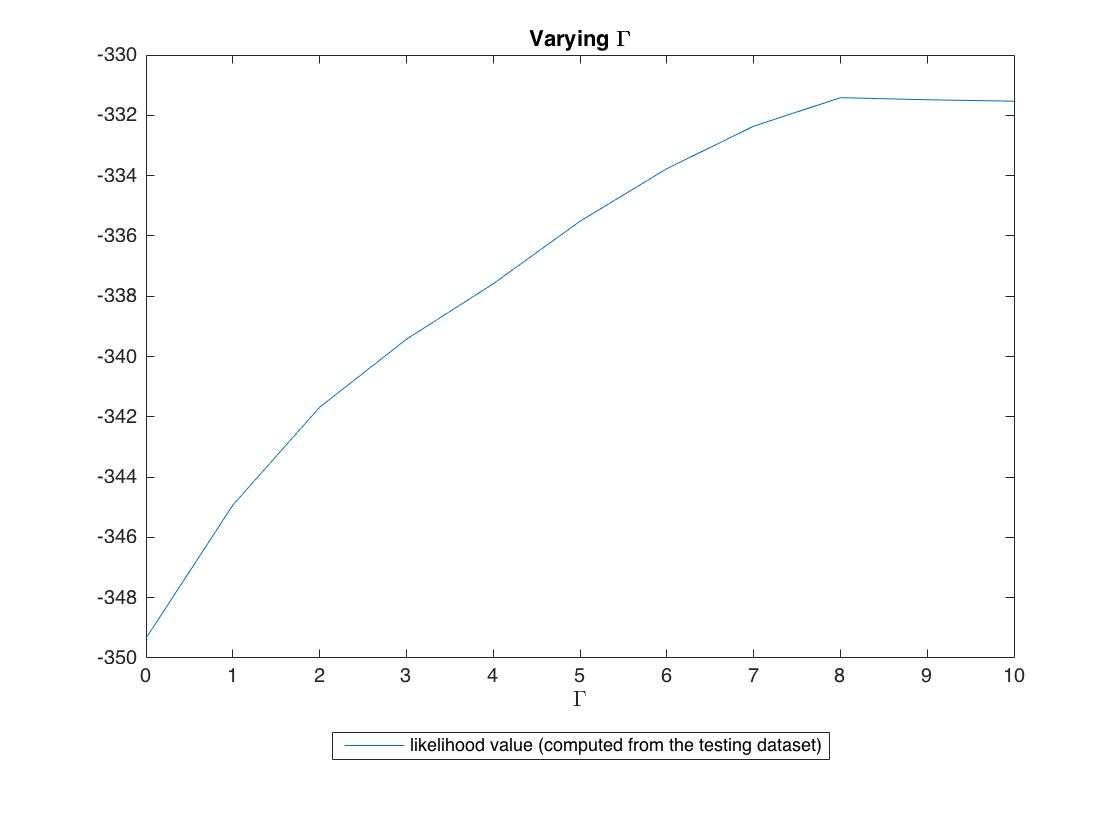
\includegraphics[scale=0.25]{vary_gamma_300_300_1_to_10}
\end{frame}

\begin{frame}
	\frametitle{Example: Robust choice model}
	\begin{itemize}
		\item When some of the data departs from the distributional assumption, a positive $\Gamma$ gives \say{better} estimates.
		\item This model has several (potential) advantages, given that the difficulty in computation is (partially) addressed.
		\begin{itemize}
			\item A systematic way to tune the parameter?
			\item How to assess \textit{goodness-of-fit}?
			\item Any theoretical justification for the improved performance?
			\item Connection to regularized regression and other models (Shafieezadeh-Abadeh, Esfahani and Kuhn, 2015)?
		\end{itemize}
	\end{itemize}
\end{frame}

\begin{frame}
	\frametitle{The algorithm}
	\begin{itemize}
		\item Recall the standard conic form (P) and consider the following pair of primal and dual problems
		\begin{align}
		\begin{split} 
		\text{Primal:} \quad &\min\,\, c^Tx\\ 
		&\textnormal{s.t.} \,\, Ax=b,\ x\in \mathcal{K} \\
		\text{Dual:}  \quad &\max\,\, b^Ty \\
		&\textnormal{s.t.} \,\, A^Ty+z=c,\ s\in\mathcal{K}^*,\ y \in \mathbb{R}^m \\
		\end{split} &\text{(PD)} \nonumber	
		\end{align}
		where $c,x \in \mathbb{R}^n$, $A\in \mathbb{R}^{m\times n}$, $b\in \mathbb{R}^m$ and $\mathcal{K} \subset \mathbb{R}^n$ is a \textit{proper} cone. Let $m\leq n$ and $\text{rank}(A) = m$. 
	\end{itemize}
\end{frame}

\begin{frame}
	\frametitle{The algorithm}
	\begin{itemize}
		\item If there exist
		$x \in \interior \left(\mathcal{K}\right)$ such that $Ax=b$ and $z \in \interior \left(\mathcal{K}^*\right)$ such that $A^Ty+z=c$,
		then \textit{strong duality} holds for (PD'). In this case, the following KKT system is necessary and sufficient for optimality of $(x,y,z)$
		\begin{align}\label{KKT_for_PD}
		\begin{split}
		Ax-b=0& \\
		A^Ty+z-c=0& \\
		x^Tz=0& \\
		x\in\mathcal{K},\ z\in \mathcal{K}^*,\ y\in\mathbb{R}^m.& 
		\end{split}
		\end{align}
	\end{itemize}
\end{frame}

\begin{frame}
	\frametitle{The algorithm}
	\begin{itemize}
		\item We introduce the (full) \textit{homogeneous self-dual embedding model} of (PD) (Ye, Todd, \& Mizuno, 1994; Toh, Todd \& T\"ut\"unc\"u, 2006),
		\begin{align*}
		\begin{split}
		& \min \,\, \bar{\alpha}\theta \\
		& \text{s.t.} \begin{bmatrix}
		0 & -A & b & -\bar b\ \\ 
		A^T & 0 & -c & \bar c \\
		-b^T & c^T& 0 & -\bar g \\
		\bar b^T & -\bar c^T & \bar g & 0
		\end{bmatrix}
		\begin{bmatrix}
		y \\ x \\ \tau \\ \theta
		\end{bmatrix} + 
		\begin{bmatrix}
		0 \\ z \\ \kappa \\ 0 
		\end{bmatrix} = 
		\begin{bmatrix}
		0 \\ 0 \\ 0 \\ \bar \alpha
		\end{bmatrix}\\
		& x \in \mathcal{K},\ z \in \mathcal{K}^*,\ \tau \geq 0,\ \kappa\geq 0,\ y \in \mathbb{R}^m,\ \theta \in \mathbb{R}, 
		\end{split} \quad \quad \quad \text{(HSD)}
		\end{align*}
		where given $(x^0, y^0, z^0, \tau^0, \kappa^0, \theta^0)$ such that $x^0 \in \interior \left(\mathcal{K}\right)$, $z^0 \in \interior \left(\mathcal{K}^*\right)$, $\tau^0, \kappa^0, \theta^0 > 0$, set
		\begin{align*}
		\bar b = \dfrac{1}{\theta^0}\left(b\tau^0 - Ax^0\right),\quad\quad  \bar c = \dfrac{1}{\theta^0}\left(c\tau^0 - A^Ty^0 - z^0\right), \\ 
		\bar g = \dfrac{1}{\theta^0}\left(c^T x^0 - b^T y + \kappa\right), \quad\quad  \bar \alpha = \dfrac{1}{\theta^0}\left((x^0)^T z^0 + \tau^0\kappa^0\right).
		\end{align*}
	\end{itemize}
\end{frame}

\begin{frame}
	\frametitle{The algorithm}
	\begin{itemize}
		\item The properties of (HSD) are summarized as follows.
			For any given $(x^0, y^0, z^0, \tau^0, \kappa^0, \theta^0)$ such that $x^0 \in \interior \left(\mathcal{K}_{\exp}\right)$, $z^0 \in \interior \left(\mathcal{P}_{\exp}\right)$ and $\tau^0, \kappa^0, \theta^0 > 0$, the auxiliary parameters $\bar{b}$, $\bar{c}$, $\bar{g}$, $\bar{\alpha}>0$ and hence (HSD) are well-defined.
			\begin{enumerate}
				\item The problem (HSD) is \textnormal{self-dual}.
				\item $(x,y,z,\tau,\kappa, \theta) = (x^0,y^0,z^0, \tau^0,\kappa^0, \theta^0)$ is a strictly feasible (primal and dual) solution.
				\item The optimal objective is always 0. 
				\item Assume $(x,y, \tau, z,\kappa, \theta)$ is feasible. Then $\theta\geq 0$ and $x^T z + \tau \kappa = \bar{\alpha} \theta$. Furthermore, the solution is optimal if and only if $\theta=0$, in which case $x^T z = \tau\kappa = 0$.
				\item Assume $(x,y, \tau, z,\kappa, 0)$ is an optimal solution. If $\tau>0$ then $(x,y,z)/\tau$ is an optimal solution to (PD). If $\kappa>0$ then either $b^Ty>0$ or $c^Tx<0$ or both hold. 
				\begin{itemize}
					\item If $b^T y>0$ then (PD) is primal-infeasible.
					\item If $c^T x < 0$ then (PD) is dual infeasible.
				\end{itemize}
				\item For any $\epsilon \geq 0$, there exists a feasible solution of (HSD) with objective value equal to $\epsilon$ (Freund, 2005).
			\end{enumerate}
	\end{itemize}
\end{frame}

\begin{frame}
	\frametitle{The algorithm}
	\begin{itemize}
		\item The goal is to find an optimal solution to (HSD).
		\item Define a \textit{central path} $\mathcal{C} = \left\{\bar x_\mu \mid \mu \in (0,1] \right\}$ that connects the initial iterate $\bar x^0 = \left(x^0,y^0,z^0,\tau^0,\kappa^0,\theta^0\right)$ (corresponding to $\mu=1$) to an optimal solution of (HSD) (corresponding to the limit point at $\mu \rightarrow 0$).
		\begin{itemize}
		\item A parametrized system of equations that characterize $\mathcal{C}$ can be established when $\mathcal{K}$ has a \textit{logarithmically homogeneous self-concordant barrier}.
		\end{itemize}
		\item The algorithm approximately traces the central path towards the direction of decreasing $\mu$.
				\begin{itemize}
					\item Based on the current iterate which is (usually) near the central path, compute the search direction by linearizing the system of equations governing the central path.
					\item The search direction is a linear combination of the predictor direction (roughly tangent to the central path) and the corrector direction (roughly normal toward the central path).
				\end{itemize}
	\end{itemize}
\end{frame}

\begin{frame}
	\frametitle{The algorithm}
	\begin{itemize}
		\item The termination conditions are (roughly) as follows. Consider a given relative accuracy $\epsilon$.
		\begin{itemize}
		\item Declare optimality and return the solution $(x,y,z)/\tau$ if
		\begin{align}
		\left\| Ax-\tau b \right\|_{\infty} &\leq \epsilon \cdot \max \left\{1, \left\|[A,b]\right\|_{\infty}\right\}, \label{P_termination}\\
		\left\|A^T y + z-c\tau\right\|_{\infty} &\leq \epsilon \cdot \max \left\{1, \left\|A^T, I , -c\right\|_{\infty}\right\},\label{D_termination}\\
		\left|c^T x/\tau - b^T y/\tau\right|  &\leq \epsilon\cdot\left(1+\left|b^T y/\tau\right|\right).\label{A_termination}
		\end{align}
		\item Declare primal and/or dual infeasibility if \eqref{P_termination}, \eqref{D_termination} and 
		\begin{align}
		\left|-c^T x+b^T y - \kappa \right| &\leq \epsilon\cdot \max \left\{1, \left\|\left[-c^T, b^T, 1\right]\right\|_{\infty}\right\}, \label{G_termination}\\
		\tau &\leq \epsilon \cdot 10^{-2} \cdot \left\{1,\kappa\right\}.\label{T_terminal}
		\end{align}
		If $b^T y>0$ ($c^T x<0$), declare primal (dual) infeasibility.
		\item Declare that the problem is ill-posed if 
		\[ \kappa \leq \epsilon \cdot 10^{-2}\cdot \min \left\{1,\tau\right\},\
		\mu \leq \epsilon \cdot 10^{-2}\cdot \mu^0.\]
		\end{itemize}
	\end{itemize}
\end{frame}

\begin{frame}
	\frametitle{Plans for the next step}
	\begin{itemize}
		\item On the algorithm and implementation.
		\begin{itemize}
				\item Incorporate warm start and iterative refinement strategies.
				\item Integrate the codes into SDPT3.
				\item Build a package that can be called by Python, Julia and so on.
				\item Try fundamentally different methods (PPA, ALM and so on) that might be less accurate but potentially more \textit{scalable}.
		\end{itemize}
		\item On application.
		\begin{itemize}
			\item Demonstrate the advantages of the robust choice model and other models that quantify distributional uncertainties.
		\end{itemize}
	\end{itemize}
\end{frame}

\begin{frame}
	\frametitle{Thank you for your attention!}
	\begin{itemize}
		\item Questions or comments?
	\end{itemize}
\end{frame}

\end{document}

